
\section{Temporal and Spatial Scopes of Update Operations}
\label{sec:scope}

The scope of an operation consists of the parts of the plan that \emph{may} be affected by the operation.

In this section, we define the scope for each of the operations defined in Section~\vref{sec:operations}. The scope is later used when creating the analysis rules for modification of the interval-based feature model.

In the section, we describe the \emph{spatial} and \emph{temporal} scopes. The spatial scope consists of the parts of a feature model that may be affected by change. For instance, adding a group affects the group being added and its parent feature, as the operation does not modify any other part of the plan. We must also take into account the \emph{temporal} aspect, since the plan also has a dimension of time. The temporal scope then consists of the time points that may be affected by applying an operation. In Figure~\vref{ex:add-group-scope}\footnote{Notice that the plan differentiates between groups and features, but does not display types or names} %TODO: readd vref but make sure it isn't at a page break.
, we visualise the spatial and temporal scopes. In the original plan, a group $D$ is added to feature $B$ at time 2. In time 3, it is moved to feature $C$. We modify the plan by adding a feature $E$ to group $D$ from time 2 to time 3. In the modified plan, the spatial and temporal scopes are shown, with the spatial scope containing group $D$ and feature $E$, and the temporal scope containing times 2 and 3. Notice that $Root$, $A$, and $B$ are not in the scope, nor are the time points 1 and 4.
\begin{figure}[h]
  \centering
      \textbf{Original plan}

      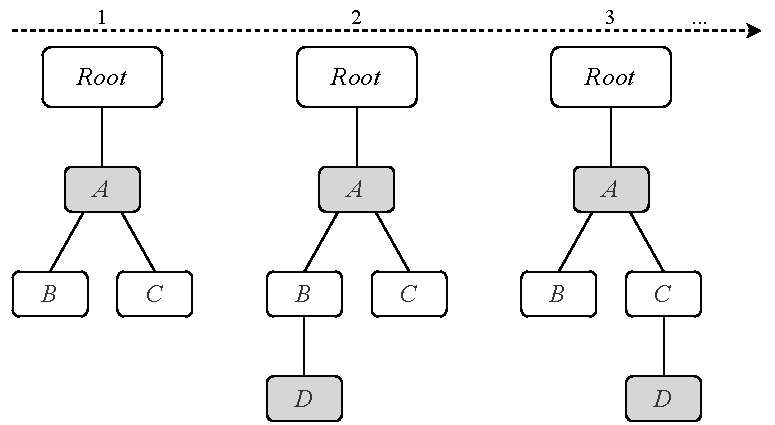
\includegraphics[width=0.6\textwidth]{MoveDPlan}
      \bigskip
      
      apply \textbf{addFeature}$(E, \ldots, D)$ from 2 to 3  
      \bigskip

      \textbf{Modified plan}

      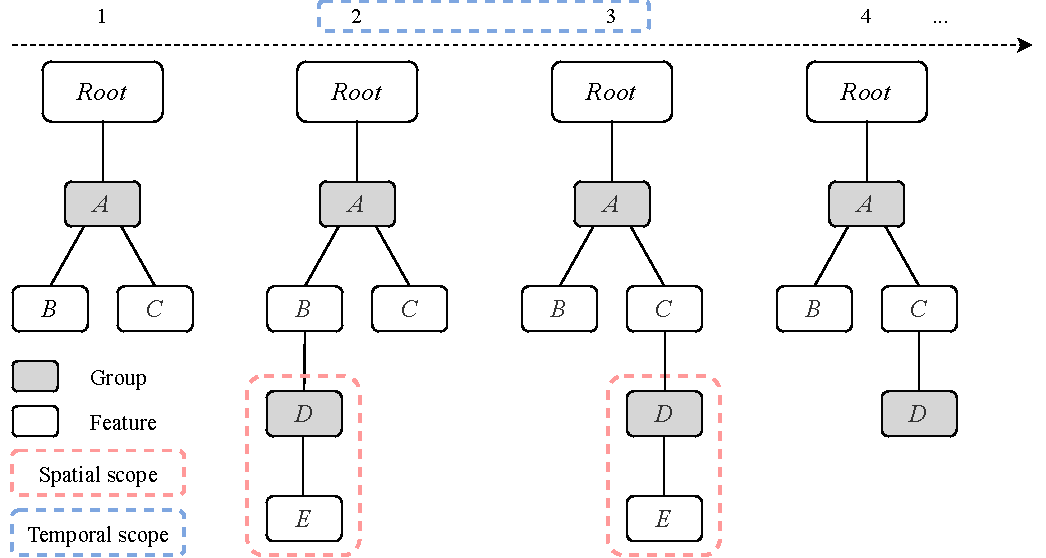
\includegraphics[width=0.8\textwidth]{MoveDPlanMod}
  \caption{Add group scope visualisation}
  \label{ex:add-group-scope}
\end{figure}

For each of the operations defined in Section~\vref{sec:operations}, we define the scope in the temporal and spatial dimensions. By assuming that the original plan is sound, meaning that it contains no paradoxes, we include only those parts of the plan in which the operation may cause a paradox.

\subsubsection*{Operation Scopes}
We define the temporal and spatial scopes for each operation.
\begin{itemize}

  \item \textbf{addFeature}(\var{featureID}, \var{parentGroupID}, \var{name}, \var{featureType}) from $t_n$ to $t_m$\\
     We argue that the temporal scope is $\interval{t_n}{t_m}$, since this is the only interval in which the plan is affected by the change. In other words, if we look at the plan as a sequence of feature models, the only models that may become invalid as a result of this modification, are the ones associated with time points between $t_n$ and (but not including) $t_m$. The spatial scope must be only the feature itself, the parent group and the name. If the group type of the parent changes to a conflicting one, the operation is unsound. If the parent group is removed, we have an orphaned feature, which is also illegal. The name is unique, so we must also verify that no other feature is using the name during the temporal scope. 
 

  \item \textbf{addGroup}(\var{groupID}, \var{parentFeatureID}, \var{groupType}) from $t_n$ to $t_m$\\
    The scopes are very similar in this and the preceding rule. The scope in time is $\interval{t_n}{t_m}$, and the scope in space is the group with id $\var{groupID}$ and the parent feature with ID $\var{parentFeatureID}$, for which the only conflicting event is removal -- the types of a group and its parent never conflict. The scope for this operation is visualised in Figure~\vref{ex:add-group-scope}
  \item \textbf{removeFeature}(\var{featureID}) at $t_n$\\
    If the original interval containing $t_n$ in which the feature exists inside the feature model is $\interval{t_m}{t_k}$, then the temporal scope is $\interval{t_n}{t_k}$, where $t_n$ is the time at which we specify that the feature be removed, and $t_k$ is the time at which the feature was \emph{originally} planned to be removed. In some cases, $t_k$ will be $\forever$, meaning that the feature was never originally planned to be removed. Since the feature is removed at $t_k$ in the original plan, and the original plan is sound as we assume, removing the feature earlier may only affect the plan in the interval between these two time points.\\
    The spatial scope must be the feature itself, its parent group, its child groups, and its name. If the feature has or will have a child group during the interval, then it cannot be removed. Otherwise, there are no conflicts. When modifying the interval-based feature model, the feature must be removed from the parent's set of child features, which is why the parent group is included in the spatial scope. Likewise, the feature's ID must be removed from its name's mappings during the temporal scope, and so the name is also inside the scope. If the name changes during the temporal scope, there is a paradox, since a feature planned to be modified should not be removed.  
  \item \textbf{removeGroup}(\var{groupID}) at $t_n$\\
    This is similar to the scope for \textbf{removeFeature}, but without consideration for names, as groups do not have names.  Thus the temporal scope is $\interval{t_n}{t_k}$, where $t_k$ is the time at which the group was originally planned to be removed. The spatial scope includes the group itself, its parent feature, and its child features. As with features, a group cannot be removed if it has or will have child features during the temporal scope.
  \item \textbf{moveFeature}(\var{featureID}, \var{targetGroupID}) at $t_n$ \\
  If $t_m$ is the time at which the feature is next moved in the original plan, the temporal scope is $\interval{t_n}{t_m}$, since this operation only affects the plan within this interval.
  \begin{figure}[h]
    \centering

      \textbf{Original plan}

      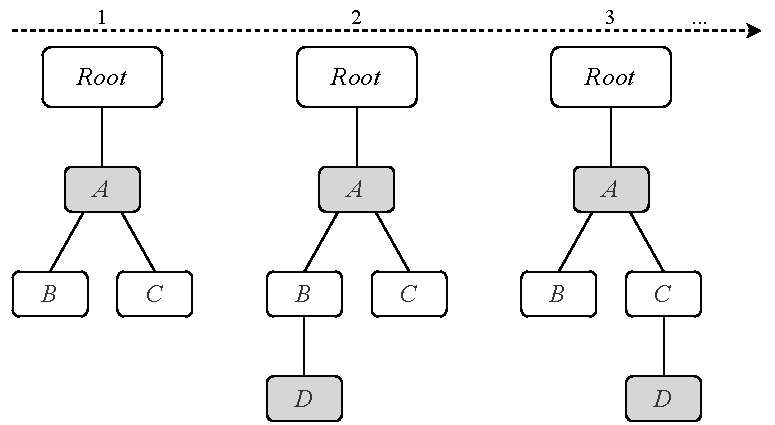
\includegraphics[width=0.7\textwidth]{MoveDPlan}
      \bigskip

      apply \textbf{moveFeature}$(C, D)$ at 2
      \bigskip

      \textbf{Modified plan}

      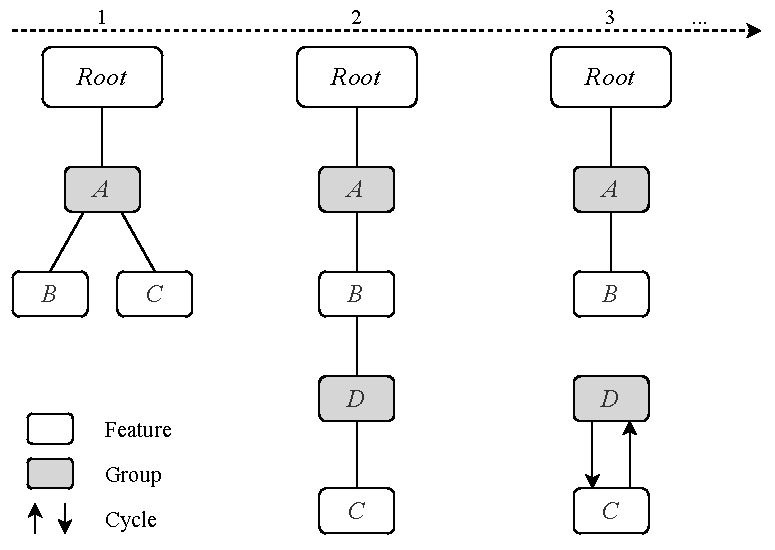
\includegraphics[width=0.7\textwidth]{CycleParadox}
    \caption{Move operation causing cycle}
    \label{ex:move-cycle}
  \end{figure}

  The spatial scope is discussed in more detail in the algorithm for moving features or groups presented in Section~\vref{sub:move-algorithm}. This scope is the largest and hardest to define, because we have to detect cycles. See Figure~\vref{ex:move-cycle} for an example of a move which causes a cycle. In the example, the original plan contains a move operation in which group $D$ is moved to feature $C$ at time 3. In the modified plan, feature $C$ is moved to group $D$ at time 2. Although this seems problem-free at time 2, it causes a paradox in the shape of a cycle at time 3, since $D$ is then moved to a group in its subtree. 

  The scope is defined by the feature and its ancestors, as well as the target group and its ancestors, which may change during the intervals due to other move operations. It is not necessary to look at all ancestors, only the ones which \var{feature} and \var{targetGroup} do not have in common in the original plan, as well as the feature and the group themselves. Conflicting types and removal of the new parent must be considered in addition to cycles.
  \item \textbf{moveGroup}(\var{groupID}, \var{targetFeatureID}) at $t_n$\\
    This is similar to the scope for \textbf{moveFeature}, as cycles violate the tree structure independently of whether the nodes are features or groups.
    The difference in spatial scope concerns types, as type conflicts can only arise between a parent group and its child feature. Since the operation does not change the relation between a parent group and its child features, and the original plan is assumed to be sound, conflicting types are not considered for this operation.
  \item \textbf{changeFeatureVariationType}(\var{featureID}, \var{newType}) at $t_n$\\
    The temporal scope is $\interval{t_n}{t_m}$ if $t_m$ is the next time point at which the feature's type changes next or when the feature is (next) removed, since this is the only part of the plan which is changed by the operation.\\
    The only possible conflict in the spatial scope is the parent group's type. At no point can the feature have type \mandatory{} and the parent group have type \xortype{} or \ortype{}. Thus, the spatial scope is the parent group and the feature itself.\\
  \item \textbf{changeGroupVariationType}(\var{groupID}, \var{newType}) at $t_n$\\
    The temporal scope is $\interval{t_n}{t_m}$ if $t_m$ is the next time point at which the group's type changes next or when the group is (next) removed, since this is the only part of the plan which is changed by the operation.

    The spatial scope includes the group's child features; the possible conflict is the same as with changeFeatureType, but between the group and its child features. Consequently, this scope may encompass several features.\\
  \item \textbf{changeFeatureName}(\var{featureID}, \var{name}) at $t_n$\\
  The temporal scope is $\interval{t_n}{t_m}$ if $t_m$ is the next time point at which the feature's name changes next or when the feature is (next) removed, since this is the only part of the plan which is changed by the operation.

    The spatial scope consists of the name, the feature, and its previous name. If it already exists within the feature model during the interval, or if the feature does not exist at time $t_n$, then the change is invalid. 
\end{itemize}

When we present the analysis, the scope is used to decide which parts of the plan need to be examined. For each operation, we analyse and modify only the parts of the plan which are inside its scope.

